% Bartosz Bednarczyk, Rafał Kaleta
% Analiza numeryczna sprawozdanie 2

\documentclass{article}

\usepackage{polski}
\usepackage[utf8]{inputenc}

\usepackage{fancyhdr} % Required for custom headers
\usepackage{lastpage} % Required to determine the last page for the footer
\usepackage{extramarks} % Required for headers and footers
\usepackage[usenames,dvipsnames]{color} % Required for custom colors
\usepackage{graphicx} % Required to insert images
\usepackage{listings} % Required for insertion of code
\usepackage{courier} % Required for the courier font
\usepackage{lipsum} 
\usepackage{amsfonts}
\usepackage{amsthm}
\usepackage{hyperref}
\usepackage{tikz}
\usepackage{amsmath}
\usepackage{pdfpages}
\usepackage{mathtools}
\usepackage{amsthm}
\usepackage{amssymb}
\usepackage{bbm}

\DeclareUnicodeCharacter{00A0}{ }

\newtheorem{thm}{Twierdzenie}
\newtheorem{remark}{Uwaga}
\newtheorem{lemat}{Lemat}
\newtheorem{wniosek}{Wniosek}
\newtheorem{definicja}{Definicja}
\newtheorem{ciekawostka}{Ciekawostka}
\newtheorem{przyklad}{Przykład}
\newtheorem{obserwacja}{Obserwacja}



\newenvironment{prooff}{\paragraph{Dowód:}}{\hfill$\square$}
\newenvironment{rozw}{\paragraph{Rozwiązanie:}}{\hfill}

\usepackage{amsfonts,graphicx}
\newcommand{\bigex}{%
\mathop{\lower0.75ex\hbox{%
   \scalebox{1.7}{\ensuremath{\exists}}}}\limits}


\usepackage{inconsolata} % very nice fixed-width font included with texlive-full
\usepackage[usenames,dvipsnames]{color} % more flexible names for syntax highlighting colors
\usepackage{listings}

\lstset{
basicstyle=\small\ttfamily, 
columns=fullflexible, % make sure to use fixed-width font, CM typewriter is NOT fixed width
numbers=left, 
numberstyle=\small\ttfamily\color{Gray},
stepnumber=1,              
numbersep=10pt, 
numberfirstline=true, 
numberblanklines=true, 
tabsize=4,
lineskip=-1.5pt,
extendedchars=true,
breaklines=true,        
keywordstyle=\color{Blue}\bfseries,
identifierstyle=, % using emph or index keywords
commentstyle=\sffamily\color{OliveGreen},
stringstyle=\color{Maroon},
showstringspaces=false,
showtabs=false,
upquote=false,
texcl=true, % interpet comments as LaTeX
    literate={á}{{\'a}}1 {ã}{{\~a}}1 {é}{{<}}1,
inputencoding=utf8
}

\lstdefinelanguage{julia}
{
  keywordsprefix=\@,
  morekeywords={
    exit,whos,edit,load,is,isa,isequal,typeof,tuple,ntuple,uid,hash,finalizer,convert,promote,
    subtype,typemin,typemax,realmin,realmax,sizeof,eps,promote_type,method_exists,applicable,
    invoke,dlopen,dlsym,system,error,throw,assert,new,Inf,Nan,pi,im,begin,while,for,in,return,
    break,continue,macro,quote,let,if,elseif,else,try,catch,end,bitstype,ccall,do,using,module,
    import,export,importall,baremodule,immutable,local,global,const,Bool,Int,Int8,Int16,Int32,
    Int64,Uint,Uint8,Uint16,Uint32,Uint64,Float32,Float64,Complex64,Complex128,Any,Nothing,None,
    function,type,typealias,abstract
  },
  sensitive=true,
  morecomment=[l]{\#},
  morestring=[b]',
  morestring=[b]" 
}

% Margins
\topmargin=-0.45in
\evensidemargin=0in
\oddsidemargin=0in
\textwidth=7in
\textheight=9.0in
\headsep=0.25in

\linespread{1.1} % Line spacing

% Set up the header and footer
\pagestyle{fancy}
\lhead{\hmwkAuthorName} % Top left header
\rhead{\firstxmark} % Top right header
\lfoot{\lastxmark} % Bottom left footer
\cfoot{} % Bottom center footer
\rfoot{Page\ \thepage\ of\ \protect\pageref{LastPage}} % Bottom right footer
\renewcommand\headrulewidth{0.4pt} % Size of the header rule
\renewcommand\footrulewidth{0.4pt} % Size of the footer rule

\setlength\parindent{0pt} % Removes all indentation from paragraphs
%----------------------------------------------------------------------------------------
%	DOCUMENT STRUCTURE COMMANDS
%	Skip this unless you know what you're doing
%----------------------------------------------------------------------------------------

% Header and footer for when a page split occurs within a problem environment
\newcommand{\enterProblemHeader}[1]{
\nobreak\extramarks{#1}{#1 continued on next page\ldots}\nobreak
\nobreak\extramarks{#1 (continued)}{#1 continued on next page\ldots}\nobreak
}

% Header and footer for when a page split occurs between problem environments
\newcommand{\exitProblemHeader}[1]{
\nobreak\extramarks{#1 (continued)}{#1 continued on next page\ldots}\nobreak
\nobreak\extramarks{#1}{}\nobreak
}

\setcounter{secnumdepth}{0} % Removes default section numbers
\newcounter{homeworkProblemCounter} % Creates a counter to keep track of the number of problems

\newcommand{\homeworkProblemName}{}
\newenvironment{homeworkProblem}[1][Zadanie \arabic{homeworkProblemCounter}]{ % Makes a new environment called homeworkProblem which takes 1 argument (custom name) but the default is "Problem #"
\stepcounter{homeworkProblemCounter} % Increase counter for number of problems
\renewcommand{\homeworkProblemName}{#1} % Assign \homeworkProblemName the name of the problem
\section{\homeworkProblemName} % Make a section in the document with the custom problem count
\enterProblemHeader{\homeworkProblemName} % Header and footer within the environment
}{
\exitProblemHeader{\homeworkProblemName} % Header and footer after the environment
}

\newcommand{\problemAnswer}[1]{ % Defines the problem answer command with the content as the only argument
\noindent\framebox[\columnwidth][c]{\begin{minipage}{0.98\columnwidth}#1\end{minipage}} % Makes the box around the problem answer and puts the content inside
}

\newcommand{\homeworkSectionName}{}
\newenvironment{homeworkSection}[1]{ % New environment for sections within homework problems, takes 1 argument - the name of the section
\renewcommand{\homeworkSectionName}{#1} % Assign \homeworkSectionName to the name of the section from the environment argument
\subsection{\homeworkSectionName} % Make a subsection with the custom name of the subsection
\enterProblemHeader{\homeworkProblemName\ [\homeworkSectionName]} % Header and footer within the environment
}{
\enterProblemHeader{\homeworkProblemName} % Header and footer after the environment
}

\usepackage{listings} % Required for inserting code snippets
\usepackage[usenames,dvipsnames]{color} % Required for specifying custom colors and referring to colors by name

\definecolor{DarkGreen}{rgb}{0.0,0.4,0.0} % Comment color
\definecolor{highlight}{RGB}{255,251,204} % Code highlight color

% Create a command to cleanly insert a snippet with the style above anywhere in the document
\newcommand{\insertcode}[2]{\begin{itemize}\item[]\lstinputlisting[caption=#2,label=#1,style=Style1]{#1}\end{itemize}} % The first argument is the script location/filename and the second is a caption for the listing

%----------------------------------------------------------------------------------------
%	NAME AND CLASS SECTION
%----------------------------------------------------------------------------------------

\newcommand{\hmwkTitle}{Pracownia 2} % Assignment title
\newcommand{\hmwkDueDate}{} % Due date
\newcommand{\hmwkClass}{Analiza numeryczna} % Course/class
\newcommand{\hmwkClassTime}{} % Class/lecture time
\newcommand{\hmwkClassInstructor}{} % Teacher/lecturer
\newcommand{\hmwkAuthorName}{Bartosz Bednarczyk, Rafał Kaleta - Sprawozdanie z pracowni nr 2 - Zadanie 21} % Your name

%----------------------------------------------------------------------------------------
%	TITLE PAGE
%----------------------------------------------------------------------------------------

\title{Analiza numeryczna (M) - Pracownia 2 - Zadanie P2.21\\
Metody konstruowania baz dualnych\\ oraz ich zastosowania w problemach numerycznych}
\date{Grudzień 13, 2015}
\author{Bartosz Bednarczyk\\ \and Rafał Kaleta}


%----------------------------------------------------------------------------------------

\begin{document}

\maketitle

\tableofcontents

\section{Krótki wstęp}

Rozwiązanie problemu wyszukiwania baz dualnych jest współcześnie bardzo pożądane. Jest to związane z faktem, że mnóstwo innych problemów matematycznych bądź informatycznych można rozwiązać za ich pomocą. Jednym z takich problemów jest znajdowanie wielomianów przybliżających inne, bardziej skomplikowane funkcje, gdyż pozwala to na znaczące uproszczenie obliczeń. Rozważania dotyczące baz dualnych nie są jednakże kwestią czysto teoretyczną. W~ostatnich czasach bazy dualne oraz wielomiany optymalne znalazły wielu zwolenników w środowiskach naukowych, gdyż mają szereg wielu ciekawych zastosowań w obliczeniach numerycznych i grafice komputerowej.\\

Tematem niniejszego sprawozdania są bazy dualne w przestrzeni funkcji z ustalonym iloczynem skalarnym oraz ich zastosowania, szczególnie w aproksymacji najróżniejszych funkcji. Przede wszystkim skupimy się na generowaniu takich baz (a to nie jest najprostsze zadanie) za pomocą kilku metod oraz na uzyskaniu wielomianu optymalnego w~sensie normy średniokwadratowej. Zobaczymy też jak bliskie aproksymowanym funkcjom są uzyskane wielomiany.

\section{Bazy dualne i metody ich wyznaczania}

\subsection{Definicja i podstawowe własności}

\begin{center}
\begin{tikzpicture}
\node [draw={black}, fill=black!10, very thick, rectangle, rounded corners, inner sep=12pt, inner ysep=12pt] (box){%
    \begin{minipage}{.9\textwidth}

	Niech $B_n = \left\{ b_0, b_1, \ldots, b_n\right\}$ będzie liniowo niezależnym układem funkcji. Rozważmy przestrzeń linową $\mathcal{B}_n = span \left\{ b_0, b_1, \ldots b_n \right\}$ wyposażoną w iloczyn skalarny $\langle\cdot,\cdot\rangle \ : \ \mathcal{B}_n \times \mathcal{B}_n \rightarrow \mathbb{R}$.\\
	
	Układ funkcji $ \lbrace d_0^{(n)}, d_1^{(n)}, \ldots, d_n^{(n)} \rbrace$ będziemy nazywać \textbf{bazą dualną}  $D_n$ przestrzeni $\mathcal{B}_n$, jeżeli:\\
	
	\begin{itemize}
	\item $\mathcal{B}_n = span \left\{ d_0^{(n)}, d_1^{(n)}, \ldots, d_n^{(n)} \right\}$ 	

	\item $\langle b_i,d_j^{(n)} \rangle = \delta_{ij}$ dla $0 \leq i, j \leq n$, gdzie $\delta_{ij}$ to delta Kroneckera.
	
	\end{itemize}
	
    \end{minipage}
};
\node[fill={black}, text=white, rounded corners, right=10pt] at (box.north west) {Definicja bazy dualnej};
\end{tikzpicture}
\end{center}

\begin{lemat}
Każdą funkcję $f_n \in \mathcal{B}_n$ można zapisać w postaci:
$$f_n = \sum_{k=0}^n \langle f_n, d_k^{(n)} \rangle \ b_k$$	
\end{lemat}

\begin{proof}
Ustalmy $n \in \mathbb{N}$. Weźmy dowolną funkcję $f_n \in \mathcal{B}_n$. Wtedy funkcja $f_n$ zapisuje się jednoznacznie w bazie $\mathcal{B}_n$ w postaci kombinacji liniowej elementów bazy, tj.
	$$\bigex_{a_0, a_1, \ldots a_n \in \mathbb{R}}  f_n = \sum_{k=0}^n a_k b_k$$
	
	Korzystając z podstawowych własności iloczynu skalarnego otrzymujemy:
	
	$$
	\sum_{k=0}^n \langle f_n, d_k^{(n)} \rangle \ b_k = \sum_{k=0}^n \langle  \sum_{j=0}^n a_j b_j, d_k^{(n)} \rangle \ b_k = \sum_{k=0}^n \sum_{j=0}^n \langle a_j b_j, d_k^{(n)} \rangle \ b_k = 
	$$
	$$
	=
	\sum_{k=0}^n \sum_{j=0}^n a_j \langle b_j, d_k^{(n)} \rangle \ b_k = \sum_{k=0}^n \sum_{j=0}^n a_j \delta_{jk} b_k = \sum_{k=0}^n a_k b_k = f_n
	$$
	
\end{proof}

\subsection{Metody konstrukcji baz dualnych}

Po zapoznaniu się z definicją bazy dualnej od razu nasuwa się pytanie: w jaki sposób można wyznaczyć taką bazę? Okazuje się, że efektywne wyznaczanie takiej bazy jest zadaniem nietrywialnym, o czym świadczą prace \cite{PWO1}, \cite{PWO2}, \cite{PGOiPWO}. Poniżej przedstawimy przegląd różnych metod rozwiązywania tego zadania, zaczynając od najgorszych pod względem złożoności algorytmów, aż po najnowsze (na dzień dzisiejszy) wyniki naukowe. 

\subsubsection{Wyliczanie baz dualnych z definicji}

Znając definicję bazy dualnej, można pokusić się o wyznaczanie jej wprost ze wzoru. Aby to zrobić wyrazimy naszą bazę dualną $D_n$ jako kombinację liniową wyjściowej bazy $B_n$, czyli:

$$d_i^{(n)} = \sum_{k=0}^n a_{ik}^{(n)} b_k \ (0 \leq i \leq n)$$

Należy więc obliczyć współczynniki $a_{ik}^{(n)}$ tak, aby spełniona była zależność $\langle b_j, d_i^{(n)} \rangle = \delta_{ij}$.

Ustalmy $i \in \mathbb{N}$ i wprowadźmy następujące oznaczenia:
$$
\mathcal{M}_{n \times n}(\mathbb{R}) \ni G(B_n) = 
\begin{pmatrix}
\langle b_0, b_0 \rangle & \langle b_0, b_1 \rangle & \ldots & \ldots & \ldots & \langle b_0, b_n \rangle \\ 
\langle b_1, b_0 \rangle & \langle b_1, b_1 \rangle & \ldots & \ldots & \ldots & \langle b_1, b_n \rangle \\  &  &  &  & \\
\vdots & \vdots & \vdots & \vdots & \vdots \\ 
\langle b_i, b_0 \rangle & \langle b_i, b_1 \rangle & \ldots & \ldots & \ldots & \langle b_i, b_n \rangle \\ 
\vdots & \vdots & \vdots & \vdots & \vdots \\ 
\langle b_n, b_0 \rangle & \langle b_n, b_1 \rangle & \ldots & \ldots & \ldots & \langle b_n, b_n \rangle \\ 
\end{pmatrix}
$$

$$\mathbb{B}^n \ni E_i \ \wedge \ [E_i]_{x} = \delta_{ix}$$
$$\mathbb{R}^n \ni A_i \ \wedge \ [A_i]_{x} = a_{ix}^{(n)}$$

Do rozwiązania mamy układ równań:
$$G(B_n) \cdot A_i = E_i $$
Jeśli macierz $G(B_n)$ jest nieosobliwa, to jednoznaczne rozwiązanie dostajemy w postaci:

$$A_i = G(B_n)^{-1} E_i$$
Wtedy współrzędne wektora $A_i$ będą szukanymi współczynnikami dla kombinacji liniowej $i$-tego wektora dla bazy dualnej. Algorytm możemy zapisać w pseudokodzie:

\begin{enumerate}
\item Oblicz $G(B_n)$.
\item Oblicz $G(B_n)^{-1}$.
\item Dla każdego $i$ od $0$ do $n$:
\begin{enumerate}
	\item Podstaw $A_i := G(B_n)^{-1} \cdot E_i$.
	\item Wypisz $d_{i}^{(n)} = \sum_{k=0}^n [A_i]_k \cdot b_k$.
\end{enumerate}	
\end{enumerate}

Powyższy algorytm jest niepraktyczny z wielu powodów. Po pierwsze, zadanie odwracania macierzy jest źle uwarunkowane i bardzo kosztowne obliczeniowo, gdyż ma złożoność  $O(n^3)$. Poza tym, mając odwróconą macierz, w~liniowym czasie obliczamy każdy z elementów bazy dualnej. Stąd algorytm ten jest rzadko używany w praktycznych zastosowaniach numerycznych.

\subsubsection{Zastosowanie baz ortonormalnych}
\label{dualnezdef}

Załóżmy, że mamy pewną bazę $B_n$ przestrzeni $\mathcal{B}_n$ wraz z iloczynem skalarnym. Taką bazę możemy zortonormalizować (np. metodą Grama-Schmidta). Mając bazę ortonormalną przestrzeni można łatwo sprawdzić, że jest ona dualna sama do siebie (co również pokażemy podczas testów komputerowych). Zatem zamiast korzystać z wyjściowej bazy, możemy korzystać z bazy ortonormalnej. Podobnie jak poprzednio, takie podejście jest niepraktyczne, gdyż ortonormalizacja bazy jest wyjątkowo kosztowna obliczeniowo, jak również dla niektórych baz źle uwarunkowana.

\subsubsection{Nowe metody wyznaczania baz dualnych}

Metody prezentowane wcześniej miały ogromne wady, gdyż ich asymptotyczna złożoność była wysoka lub wymagały dodatkowych informacji, jak np. znajomość bazy ortonormalnej. Poniżej przedstawimy rozwiązanie korzystające z~algorytmu iteracyjnego wyznaczania baz dualnych.\\

Mamy daną bazę $B_n = \lbrace b_0, b_1, \ldots, b_n \rbrace $ i będziemy konstruować bazę $$D_n = \lbrace d_0^{(n)}, d_1^{(n)}, \ldots, d_n^{(n)} \rbrace$$ dualną do $B_n$.\\

Rozważmy bazę $B_m = \lbrace b_0, b_1, \ldots, b_m \rbrace $ dla $0 \leq m < n$, dla której znamy bazę dualną $D_m = \lbrace d_0^{(m)}, d_1^{(m)}, \ldots, d_m^{(m)} \rbrace$.

Zauważmy, że dla $m = 0$ mamy $$D_0 = \lbrace d_0^{(0)} \rbrace, \  \text{gdzie} \  d_0^{(0)} = \langle b_0, b_0 \rangle^{-1} b_0$$ Pokażmy teraz jak wyznaczyć bazę $D_{m+1}$ dualną do $B_{m+1}$. Wówczas zachodzi $span \left( D_{m+1} \right)  =  span \left( B_{m+1} \right)$\\ oraz dla dowolnych $0 \leq i, j \leq m+1$ zachodzi $\langle b_i , d_j^{(m+1)}\rangle = \delta_{ij}$.\\

Chcemy wyznaczyć funkcje dualne $d_j^{(m+1)}$ dla $0 \leq j \leq m+1$ mające postać:
 
 $$
 d_j^{(m+1)} = \sum_{k=0}^{m} c_{jk}^{(m+1)} \ \cdot \ d_k^{(m)} + c_{j, m+1}^{(m+1)} \ \cdot \ b_{m+1} \ (0 \leq j \leq m+1),
 $$
 
 gdzie współczynniki $c_{jk}^{(m+1)}$ są wyznaczone zgodnie z warunkiem dualności bazy.\\ Współczynniki $c_{jk}^{(m+1)}$ spełniają układ równań:
 
 $$
 \begin{pmatrix}
1 & 0 & \ldots & 0 & \ldots & 0 & \langle b_{0}, b_{m+1} \rangle \\ 
0 & 1 & \ldots & 0 & \ldots & 0 & \langle b_{1}, b_{m+1} \rangle \\ 
\vdots & \vdots & \ddots & \vdots & \ddots & \vdots &  \vdots \\ 
0 & 0 & \ldots & 1 & \ldots & 0 & \langle b_{j}, b_{m+1} \rangle \\ 
\vdots & \vdots & \ddots & \vdots & \ddots & \vdots & \vdots \\ 
0 & 0 & \ldots & 0 & \ldots & 1 &  \langle b_{m}, b_{m+1} \rangle \\ 
\langle b_{m+1}, d_0^{(m)} \rangle & \langle b_{m+1}, d_1^{(m)} \rangle & \ldots & \ldots & \ldots & \langle b_{m+1}, d_m^{(m)} \rangle & \langle b_{m+1}, b_{m+1} \rangle
\end{pmatrix} \cdot \begin{pmatrix}
c_{j0}^{(m+1)} \\ 
c_{j1}^{(m+1)}\\ 
c_{j2}^{(m+1)}\\ 
\vdots \\ 
\vdots \\ 
c_{jm}^{(m+1)}\\
c_{j,m+1}^{(m+1)}\\ 
\end{pmatrix} =\begin{pmatrix}
0 \\ 
0\\ 
0\\ 
\vdots \\ 
1 \\ 
0\\
\vdots\\
0 
\end{pmatrix}  $$

W pracy \cite{PWO1} pokazano, że taki układ można rozwiązać w czasie liniowym, a powyższa macierz może być odwrócona w~czasie $O(n^2)$. Szczegóły dowodu tych faktów pozostawiamy do doczytania Czytelnikowi w podanej pracy. Podsumowując, w powyższym algorytmie potrafimy iteracyjnie wyznaczać bazy dualne bez wiedzy o bazach ortonormalnych ani wyliczania dość kosztownych macierzy odwrotnych. Sumarycznie dostajemy algorytm o złożoności $O(n^3)$, gdyż iteracyjnie musimy wyznaczyć $n$ elementów bazy, a koszt obliczenia każdego z nich wynosi $O(n^2)$

\subsubsection{Usprawniony algorytm}

Okazuje się, że do wyznaczenia bazy dualnej nie jest konieczne korzystanie z macierzy lub ich odwracanie. Podobnie jak poprzednio chcemy wyznaczyć bazę dualną $D_n$. Załóżmy, że udało się nam poznać bazę $D_m$ dualną do $B_m$ dla $0 \leq m < n$ i poszukujemy bazy $D_{m+1}$.

\begin{thm}
Elementy baz dualnych $D_m$ oraz $D_{m+1}$ spełniają dla każdego $0 \leq j \leq m$ równość
$$
d_j^{(m)} = d_j^{(m+1)} + \langle b_{m+1} , d_j^{(m)} \rangle \cdot d_{m+1}^{(m+1)}
$$
\end{thm}

\begin{proof}
Dostępny w \cite{PWO2} na stronie $303$.	
\end{proof}

Zauważmy, że $d_j^{(m+1)} = d_j^{(m)} - \langle b_{m+1} , d_j^{(m)} \rangle \cdot d_{m+1}^{(m+1)}$. Stąd widać, że znając bazę dualną $D_m$ możemy wyznaczyć bazę $D_{m+1}$. Jedyne co musimy wyliczyć to $d_{m+1}^{(m+1)}$, ale możemy zrobić to za pomocą poprzedniego algorytmu.

\pagebreak

Z pracy \cite{PWO1} wiemy, że 

$$
d_{m+1}^{(m+1)} = \sum_{k=0}^n \left( \frac{\langle b_k, b_{n+1} \rangle}{t_{n+1}} \cdot d_{k}^{(n)} \right) + \frac{1}{t_{n+1}} \cdot b_{n+1}, \ \text{gdzie} \ t_{n+1} = \langle b_{n+1}, b_{n+1} \rangle - \sum_{k=0}^n \langle b_{n+1}, d_{k}^{(n)} \rangle \cdot \langle b_k, b_{n+1} \rangle
$$

Zatem możemy w czasie liniowym wyznaczyć element $d_{n+1}^{(n+1)}$, dzięki czemu możemy wyznaczyć wszystkie pozostałe elementy bazy dualnej $D_{n+1}$ za pomocą powyższych wzorów również w czasie liniowym. Podsumowując, usprawniony algorytm ma złożoność $O(n^2)$, czyli aż o rząd lepiej niż poprzednio.

\section{O kilku ciekawych problemach (z bazami dualnymi w tle)}

\subsection{Konstrukcja dualnej funkcji B-sklejanej}

Krzywą sklejaną złożoną z wielomianów w reprezentacji B-sklejanej będącej uogólnioną reprezentacją krzywych Beziera nazywamy krzywą B-sklejaną. Określa się ją poprzez podanie ciągu węzłów i punktów kontrolnych na płaszczyźnie. Krzywe B-sklejane znajdują zastosowanie w modelowaniu figur o wysokim stopniu skomplikowania, dzięki czemu unika się najróżniejszych kłopotów natury implementacyjnej.\\

Przykładową krzywą B-sklejaną przedstawiamy poniżej.\\

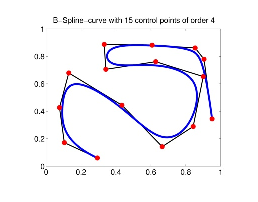
\includegraphics[width=6cm]{splajn}

Bazy dualne znajdują zastosowanie w konstrukcji dualnych funkcji B-sklejanych.\\ Zainteresowanych Czytelników zapraszamy do zapoznania się z artykułem \cite{PWO2}.

\subsection{Wielomiany Bernsteina}

Wielomiany Bersteina są ważnym typem wielomianów używanych w analizie numerycznej. W związku z tym bazy dualne do bazy złożonej z wielomianów Bersteina były często badane przez naukowców. Informacje na temat konstrukcji dualnych baz Bernsteina oraz ich zastosowanie w grafice można znaleźć w pracy \cite{PWOiSLE}.  

\subsection{Obniżanie stopnia krzywych Beziera}

Krzywe Beziera to jeden z podstawowych rodzajów krzywych występujących w matematyce i technice. Dzięki nim można przedstawiać złożone obrazy w prosty sposób. Niestety praktyka pokazuje, że krzywe Beziera mogą osiągać zbyt wysoki stopień, co znacząco utrudnia korzystanie z nich. Dlatego chcielibyśmy umieć obniżyć stopień wyjściowej krzywej za pomocą aproksymacji krzywymi Beziera o mniejszych stopniach. Do tego celu przydatne okazują się być bazy dualne, o czym można przeczytać w pracy \cite{PGOiPWO}. 

\pagebreak

\subsection{Wyszukiwanie wielomianu optymalnego w sensie normy średniokwadratowej}

\begin{lemat}
Niech $g$ będzie pewną funkcją zapisaną w bazie $\mathcal{B}_n$. Wtedy

$$
f_n^{\star} = \sum_{k=0}^n \langle g,  d_i^{(n)} \rangle \ b_i
$$

jest najlepszym przybliżeniem funkcji $g$ w sensie aproksymacji średniokwadratowej.

\end{lemat}

\begin{proof}
Prosty dowód obliczeniowy powyższego faktu pozostawiamy Czytelnikowi.	
\end{proof}

Aproksymacja funkcji wielomianami jest jedną z najszerzej wykorzystywanych technik numerycznych. Znajduje ona szereg najróżniejszych zastosowań m.in. w całkowaniu numerycznym czy przybliżanie danych uzyskanych w wyniku eksperymentów praktycznych (odszumianie sygnałów, regresja liniowa i nieliniowa, redukcja wielowymiarowości opisu danych). Jest to wyjątkowo ważne zagadnienie, więc postanowiliśmy sprawdzić jak dobre przybliżenia funkcji można uzyskać za pomocą baz dualnych (zgodnie z lematem 2). O wynikach naszych eksperymentów można przeczytać w~rozdziale poniżej.




\section{Testy numeryczne}

\subsection{Uwagi techniczne}

W celu dokładniejszego porównania powyższych wariantów metody wyszukiwania baz dualnych oraz dokładności aproksymacji funkcji z użyciem baz dualnych wykonane zostały obliczenia komputerowe. Załączony do sprawozdania program znajdował bazy dualne dla przykładowych przestrzeni liniowych wykorzystując wskazane algorytmy z~artykułów \cite{PWO1} - oznaczony w programie jako algorytm $1$ oraz z artykułu \cite{PWO2} - oznaczony w programie jako algorytm $2$. Zaimplementowaliśmy  również naiwną metodę wyszukiwania bazy dualnej za pomocą macierzy Grama, którą umieściliśmy w programie pod nazwą algorytm $0$. W każdym z rozważanych przykładów iloczyn skalarny $ \langle f, g \rangle $ obliczany był jako $$ \int_{-1}^{1} w(x) \cdot f(x) \cdot g(x) \ dx, \ \text{gdzie} \ w(x)  \ \text{to funkcja wagowa zależna od bazy}.$$ Programy zostały napisane w języku Julia 0.4 w środowisku Linux i kompilowane za pomocą polecenia \\ \textbf{julia program.jl} w terminalu. W programie używamy wbudowanej funkcji całkującej \textbf{quadgk}, o której można przeczytać w dokumentacji języka.		

\subsection{Wyniki testów komputerowych}

Testy obliczeniowe były wykonywane na czterech zestawach testowych - w każdym z nich użyto innej bazy przestrzeni wielomianów. W każdym zestawie testów aproksymowano dwie różne funkcje. Opis rodzajów testów przedstawiliśmy w tabeli poniżej:
\begin{table}[h!]
\centering
\caption{Testy}
\label{my-label}
\begin{tabular}{|c|c|c|c|c|}
\hline
Zestaw & Nazwa bazy                   & Przestrzeń & Pierwsza fun. przybliżana & Druga fun. przybliżana \\ \hline
1        & Standardowa                  & $\Pi_5$                & $\cos(x)$                    & $7x^3 + 4x^2 - 13$        \\ \hline
2        & Zaburzona standardowa        & $\Pi_4$                & $x^{\frac{2}{3}}$            & $7x^3 + 4x^2 - 13$        \\ \hline
3        & Nieznormalizowana Legendre'a & $\Pi_3$                & $\sqrt{e^x}$                 & $\sin(x^3 + 8)$           \\ \hline
4        & Znormalizowana Legendre'a    & $\Pi_3$                & $\sqrt{e^x}$                 & $x \cdot \sin(e^x) - 176$ \\ \hline
\end{tabular}
\end{table}

\begin{remark}
Poprzez zaburzoną bazę standardową rozumiemy bazę $$B = \lbrace 1, \ x-1, \ x^2 - x + 1, \ x^3 - x^2 + x - 1, \ x^4 - x^3 + x^2 - x + 1 \rbrace.$$	
\end{remark}


\begin{figure}[h!]
	\centering
	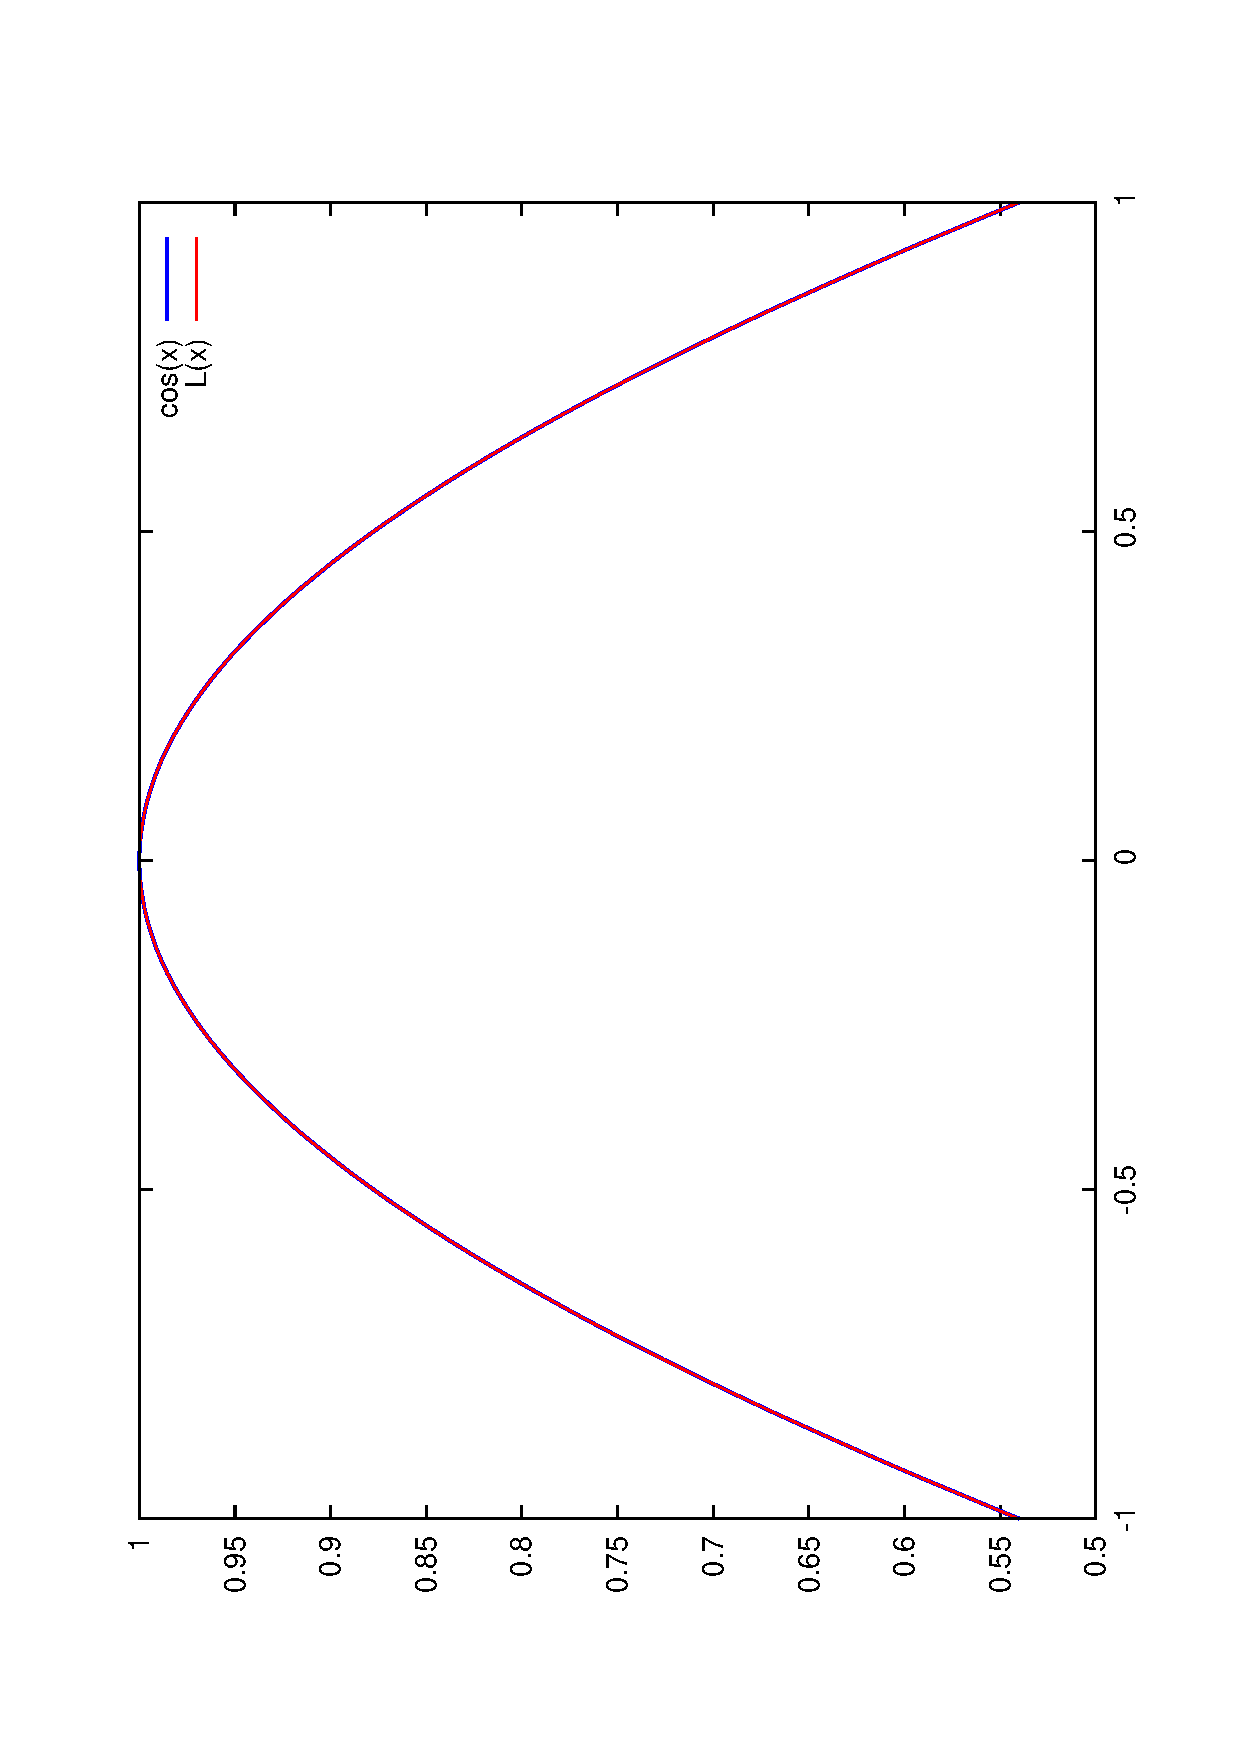
\includegraphics[width=8cm, angle = -90]{test1A}
	\caption{Przybliżenie funkcji $\cos(x)$ w bazie standardowej przestrzeni $\Pi_5$. }
\end{figure}

\begin{figure}[h!]
	\centering
	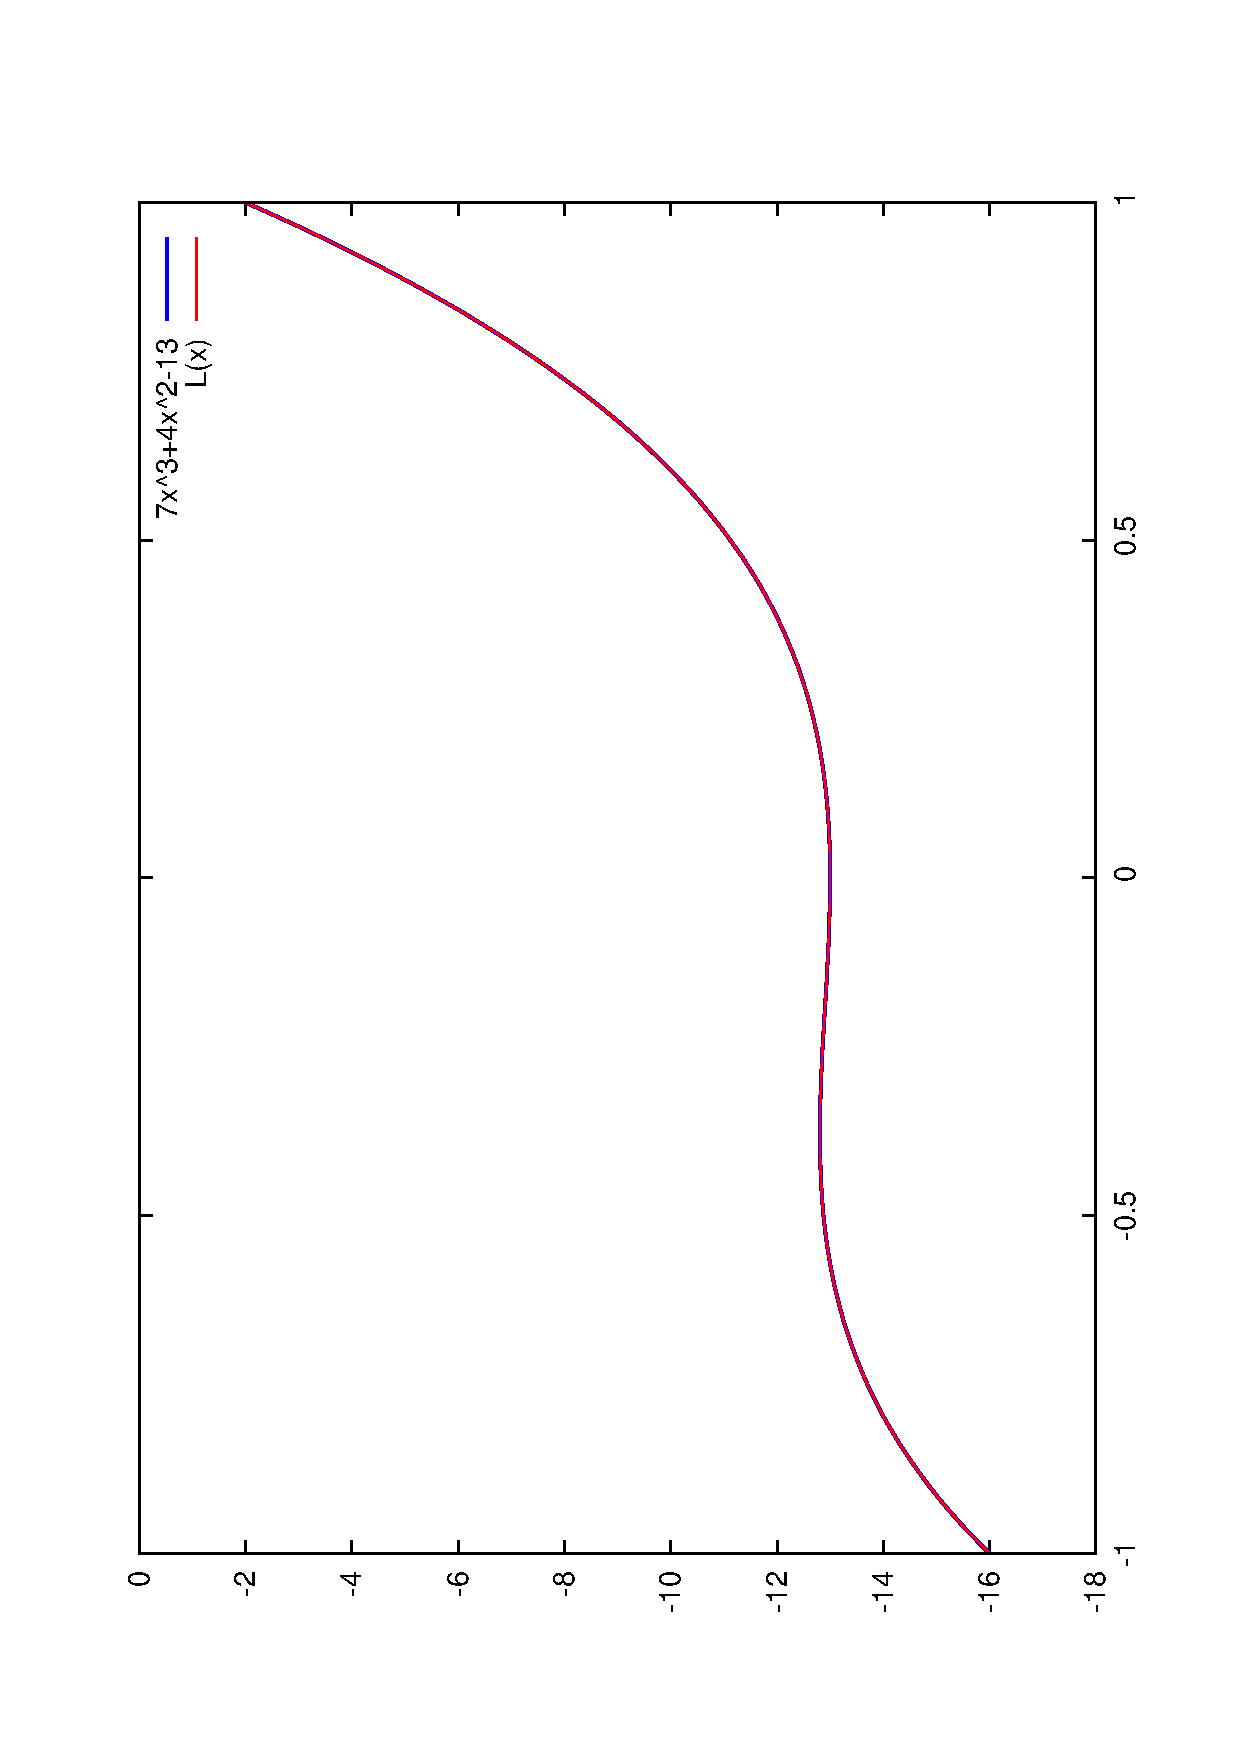
\includegraphics[width=8cm, angle = -90]{test1B}
	\caption{Przybliżenie funkcji $7x^3 + 4x^2 - 13$ w bazie standardowej przestrzeni $\Pi_5$. }
\end{figure}

\begin{obserwacja}
Podane wykresy na przedziale $[-1;1]$ funkcji niemal się pokrywają.\\ Norma średniokwadratowa funkcji błędu wyrażana jako $$\left \| f(x) - L(x) \right \|_2 = \sqrt{ \langle f(x) -L(x), f(x) -L(x) \rangle }$$
wynosi dla $y = cos(x)$ i $y = 7x^3 + 4x^2 - 13$ odpowiednio $1.3318 \cdot 10^{-9}$ oraz $8.7257 \cdot 10^{-26} \approx 0$  
\end{obserwacja}

\pagebreak

\begin{figure}[h!]
	\centering
	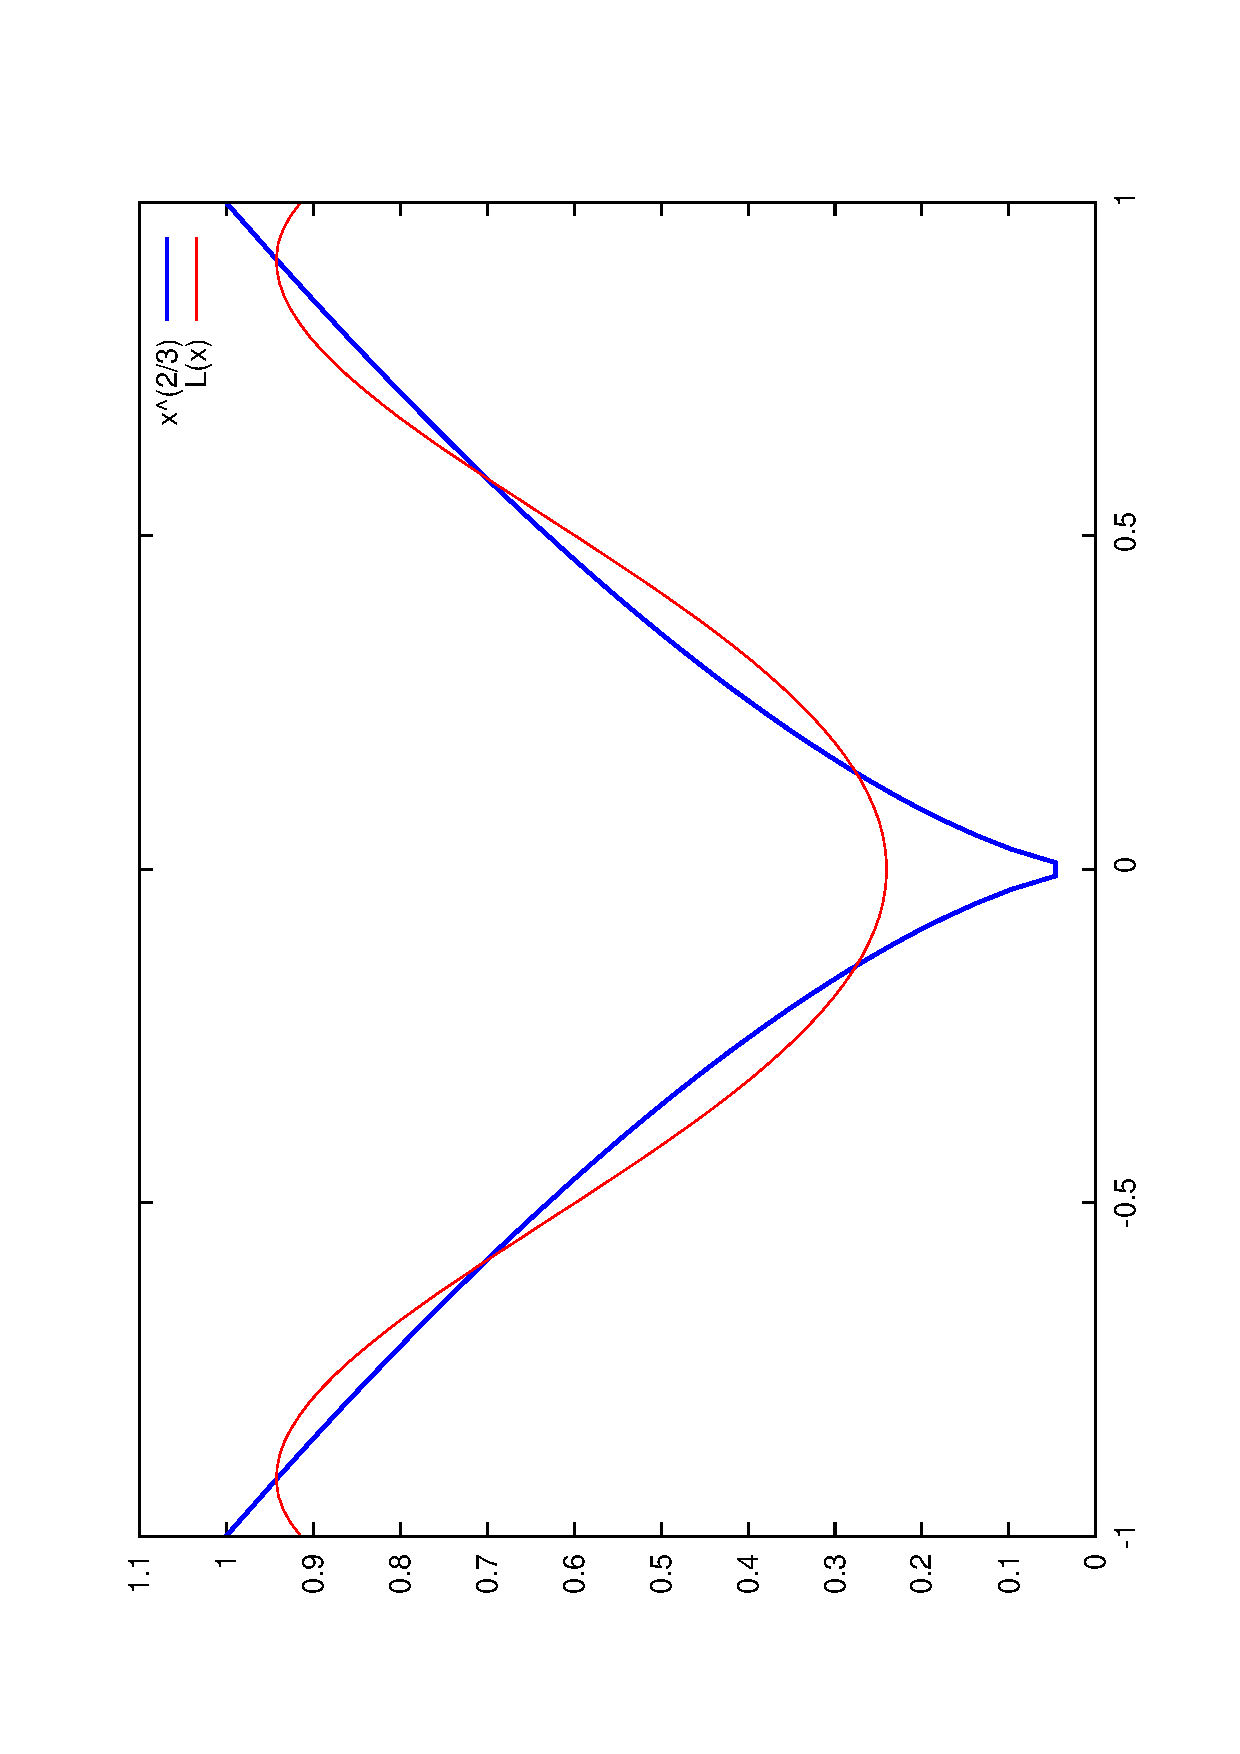
\includegraphics[width=8cm, angle = -90]{test2A}
	\caption{Przybliżenie funkcji $x^{2/3}$ w zaburzonej bazie standardowej przestrzeni $\Pi_4$. }
\end{figure}

\begin{figure}[h!]
	\centering
	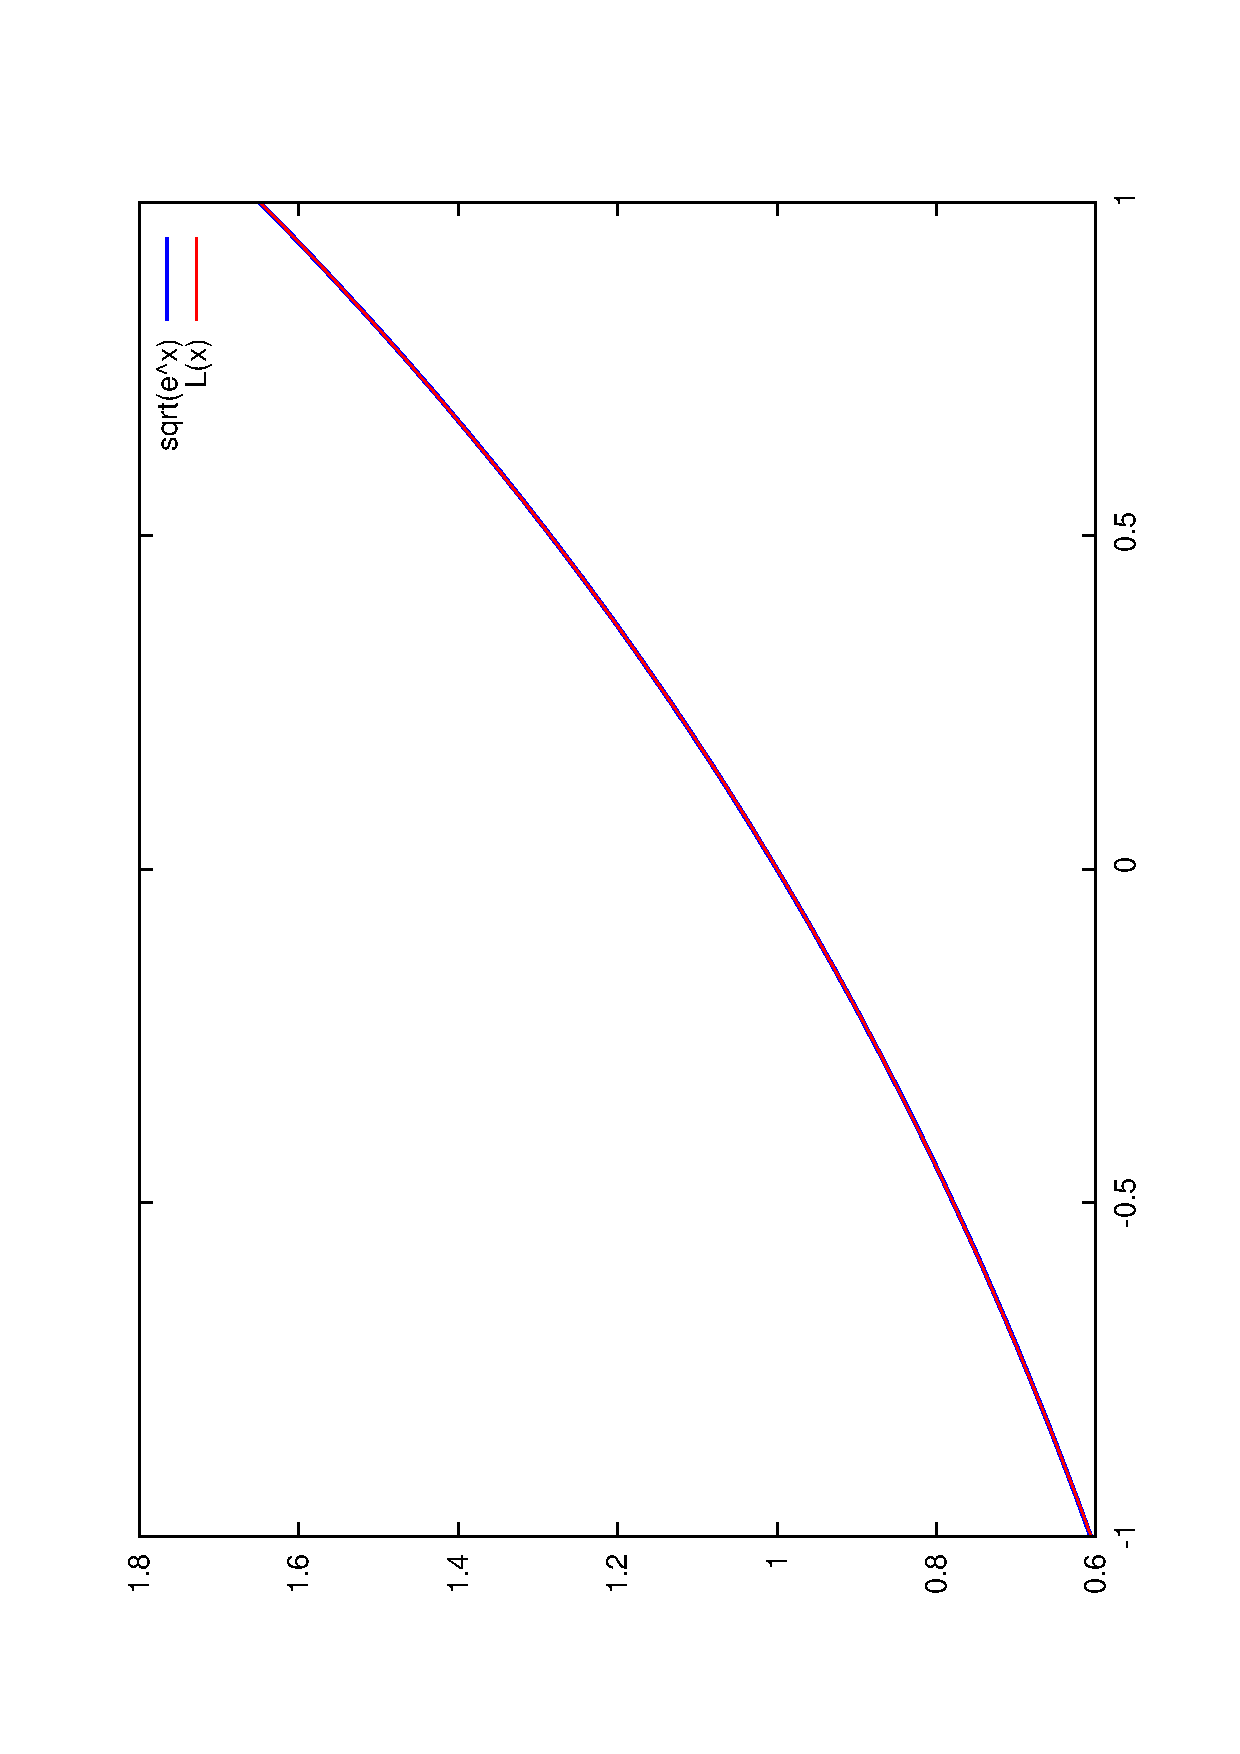
\includegraphics[width=8cm, angle = -90]{test3A}
	\caption{Przybliżanie funkcji $\sqrt{e^x}$ w nieznormalizowanej bazie Legendre'a przestrzeni $\Pi_3$}
\end{figure}

\begin{obserwacja}
Na rysunku nr $4$ możemy zauważyć, że funkcje również się pokrywają (norma błędu to $8.07466 \cdot 10^{-8}$). Natomiast na trzecim wykresie można zaobserwować dość duży błąd bezwzględny przybliżenia w okolicach zera, a wraz ze wzrostem odległości argumentów od zera błąd maleje. W tym wypadku norma wynosi w przybliżeniu $0.0063$. Przypuszczamy, że błąd w okolicach zera ma znaczący wpływ na wielkość podanej normy błędu.
\end{obserwacja}

\pagebreak

\begin{figure}[h!]
	\centering
	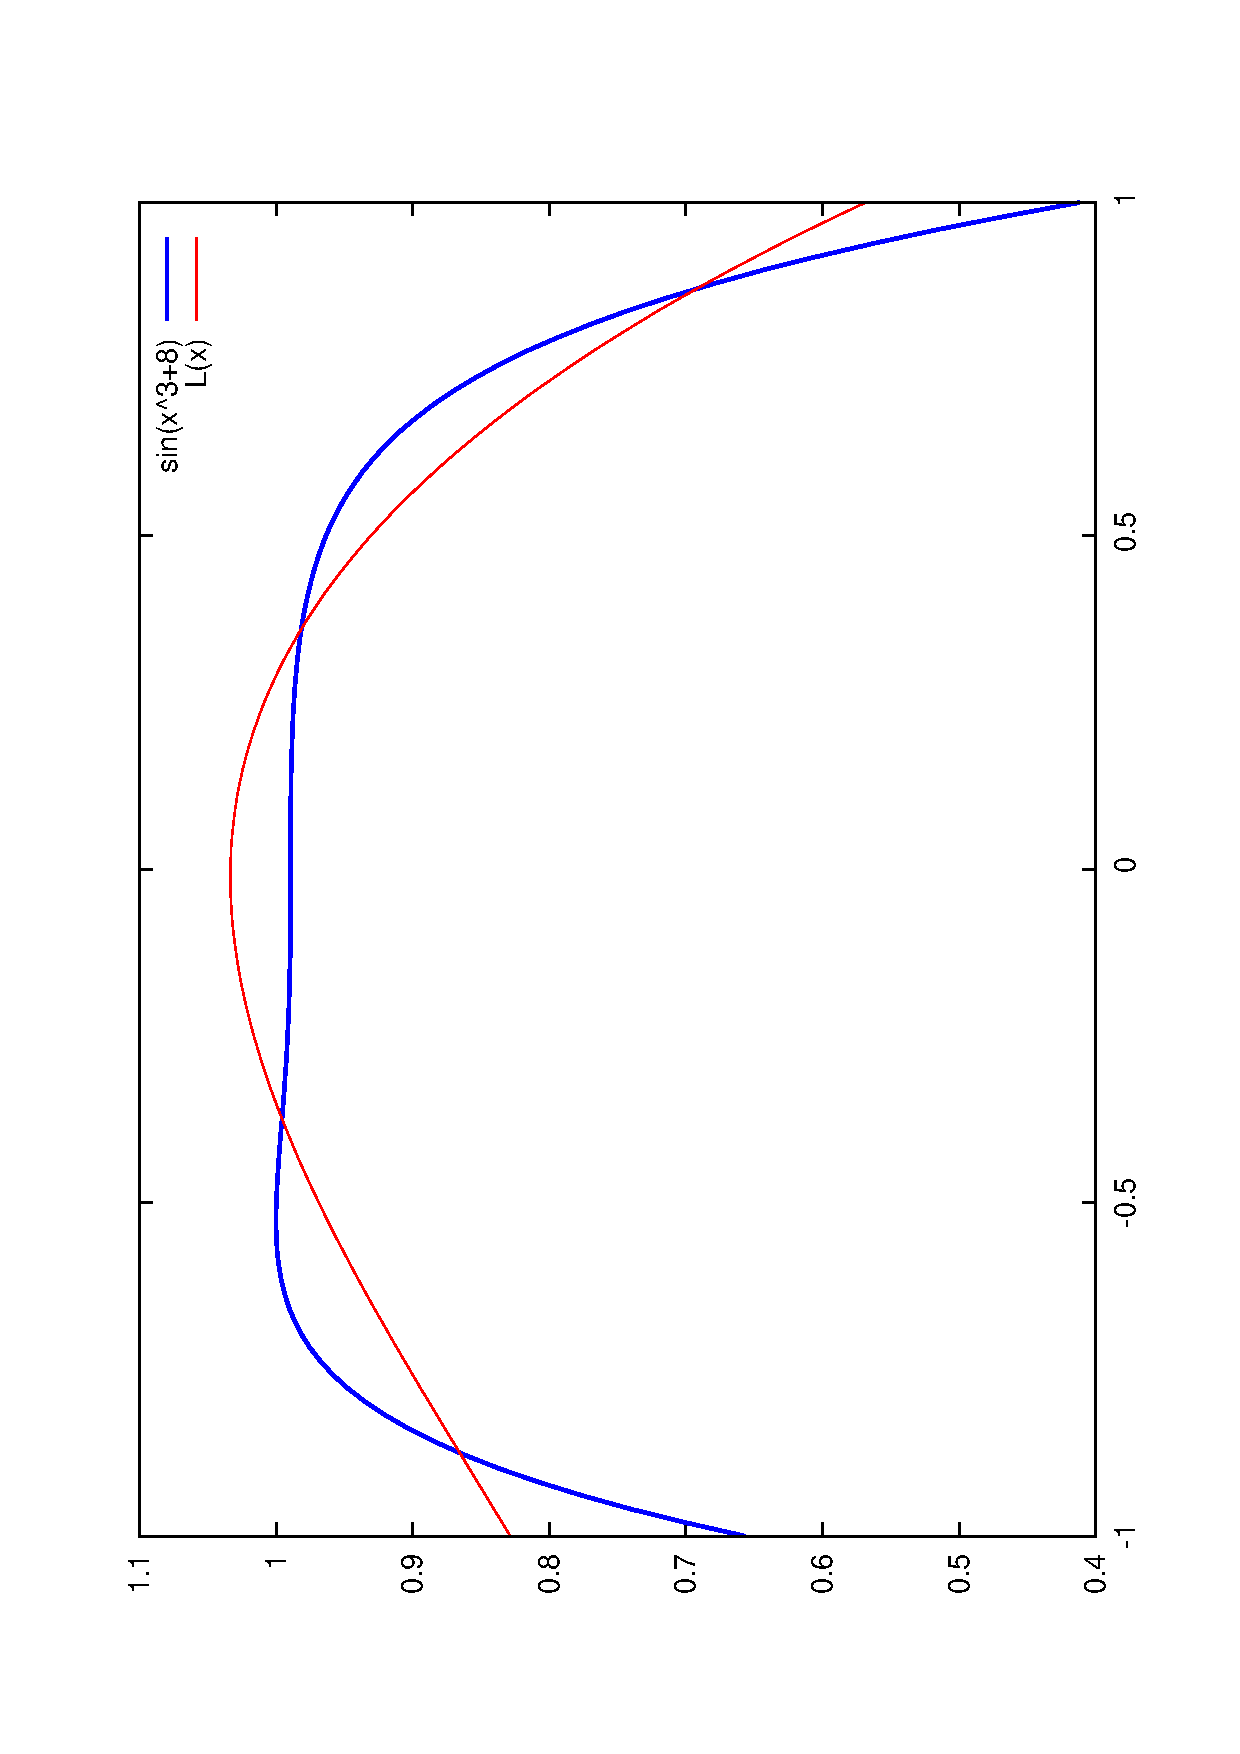
\includegraphics[width=8cm, angle = -90]{test3B}
	\caption{Przybliżanie funkcji $\sin(x^3+8)$ w nieznormalizowanej bazie Legendre'a przestrzeni $\Pi_3$}
\end{figure}

\begin{figure}[h!]
	\centering
	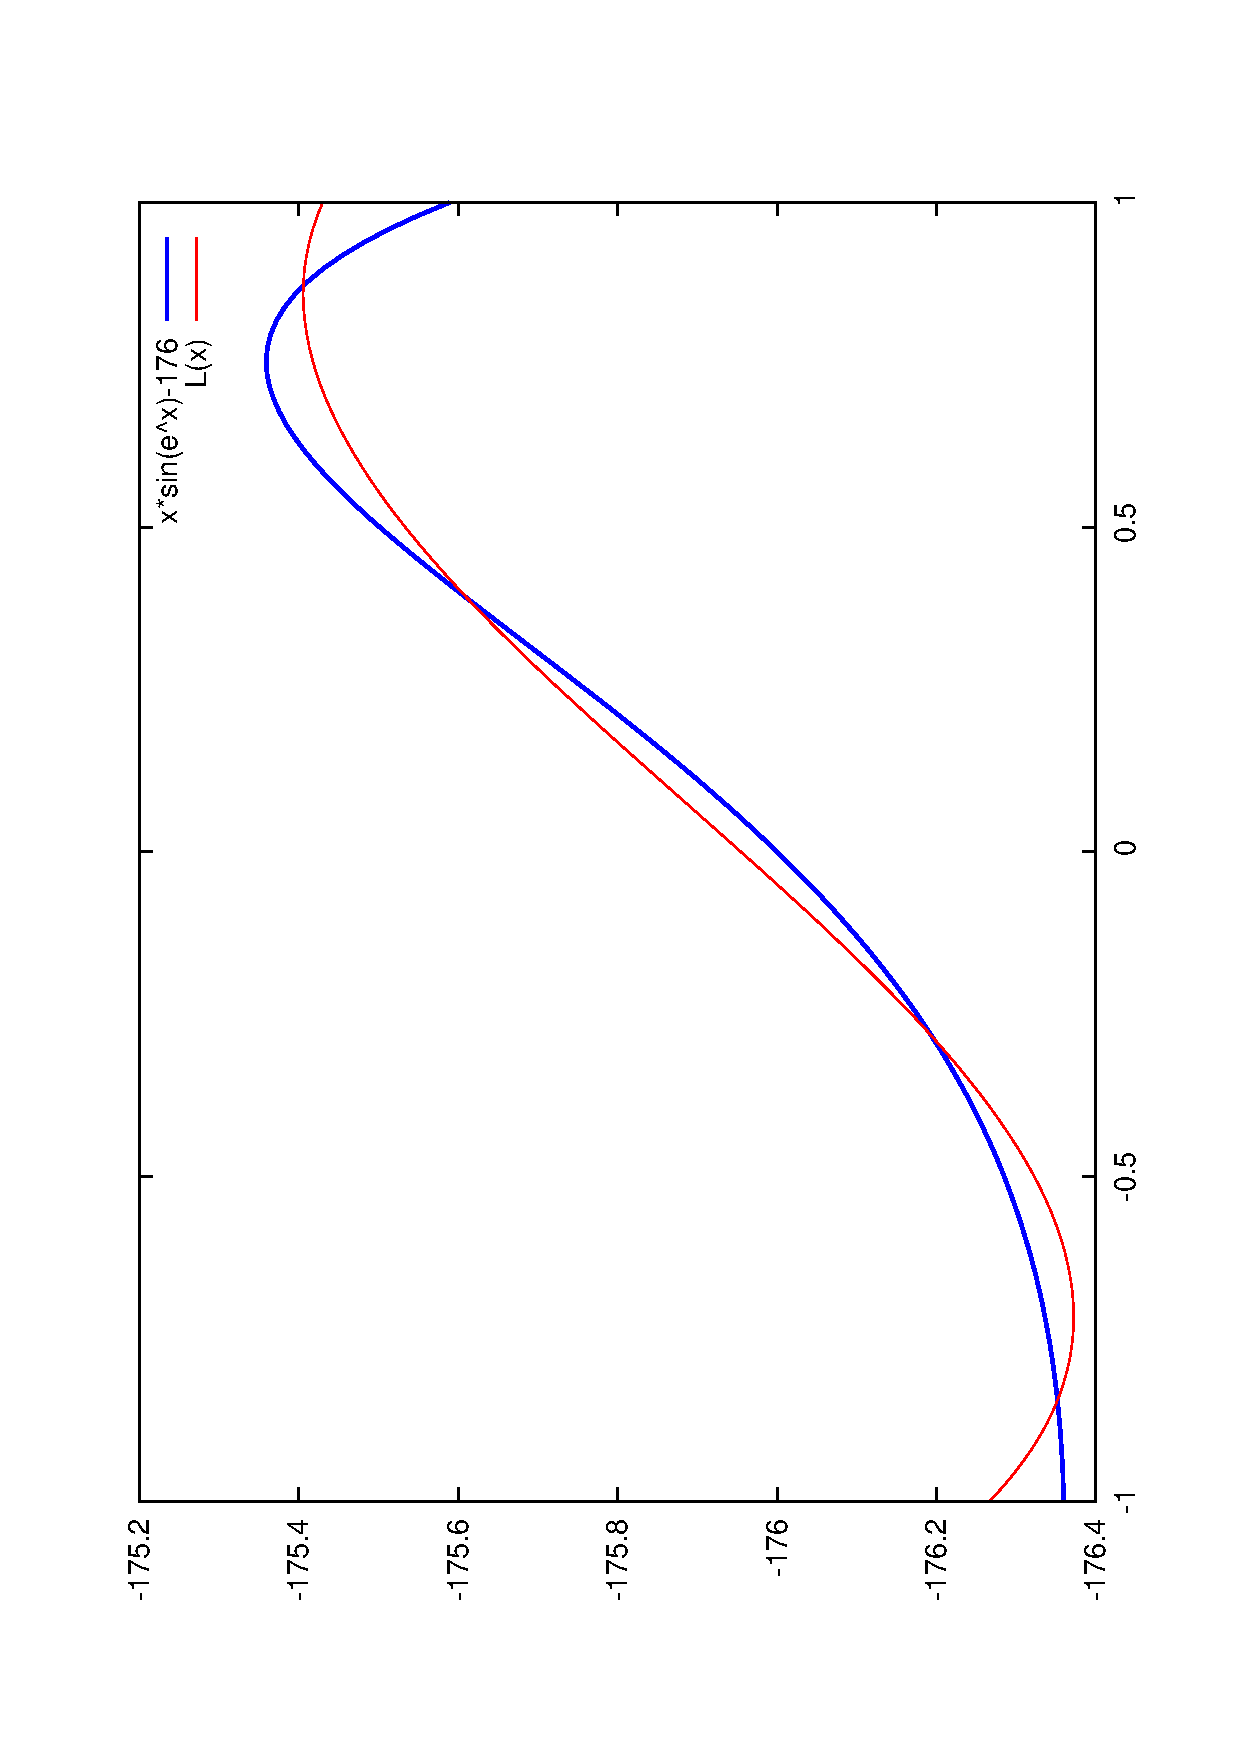
\includegraphics[width=8cm, angle = -90]{test4B}
	\caption{Przybliżanie funkcji $x \cdot \sin(e^x)-176$ w znormalizowanej bazie Legendre'a przestrzeni $\Pi_3$}
\end{figure}

\begin{obserwacja}	
Powyższe wielomiany optymalne (dla wykresów 5 i 6) wyliczane w bazach ortogonalnych wykazują typową dla aproksymacji cechę: funkcja błędu zmienia znak $5$ razy (czyli dokładnie $n+2$ razy, gdzie $n$ to stopień wielomianu). Gdybyśmy chcieli uzyskać jeszcze lepsze przybliżenie (w sensie aproksymacji jednostajnej) to możemy wybrać $n+2$ punkty, które byłyby dobrymi punktami startowymi dla algorytmu Remeza. Przypuszczamy, że wielomian optymalny w sensie normy jednostajnej dla przestrzeni z bazą ortogonalną nie różni się dużo od wielomianu optymalnego w sensie normy średniokwadratowej.
\end{obserwacja}

\subsection{Obliczenie baz dualnych}

Wyliczone bazy dualne są niemalże identyczne dla każdego z zastosowanych algorytmów. 
Różnice między uzyskanymi wynikami spowodowane są głównie błędami związanymi z przybliżaniem całki podczas obliczenia iloczynu skalarnego, a nie wyborem metody. Nie wpływają one jednak na jednoznaczne wyznaczenie wielomianów bazy dualnej. Jednakże dokładność współczynników tychże wielomianów zależy od własności numerycznych bazy wyjściowej. Największą uzyskujemy przy bazie ortogonalnej Legendre'a (w szczególności ortonormalnej), co wynika z przytoczonych faktów, że baza ortogonalna jest dualna sama do siebie (z dokładnością do stałych mnożników).

\section*{Podsumowanie}

Udało nam się poprawnie zaimplementować każdą z przedstawionych metod wyliczenia baz dualnych. Nasze wyniki są zgodne z naszymi oczekiwaniami i tylko w niewielkim stopniu odbiegają od przewidywań teoretycznych. Zastosowanie baz dualnych istotnie przyspieszyło i usprawniło obliczenia komputerowe. 

\begin{thebibliography}{99}

\bibitem{PWO1} P. Woźny,
\emph{Construction of dual bases},
Journal of Computational and Applied Mathematics 245 (2013), 75–85.

\bibitem{PWO2} P. Woźny,
\emph{Construction of dual B-spline functions},
Journal of Computational and Applied Mathematics 260 (2014), 301–311.

\bibitem{PWOiSLE} P. Woźny, S. Lewanowicz
\emph{Multi-degree reduction of Bezier curves with constraints, using dual Bernstein basis polynomials}
Computer Aided Geometric Design 26 (2009), 566–579.

\bibitem{PGOiPWO} P.Woźny, P. Gospodarczyk
\emph{A new property of dual bases and its application},
arXiv:1511.08264v1.

\bibitem{kincaid} David Kincaid, Ward Cheney, przekł. Stefan Paszkowski,
\emph{Analiza numeryczna},
Warszawa, WNT, 2006.

\bibitem{kostrikin} Aleksiej I. Kostrikin, przekł. Jerzy Trzeciak,
\emph{Wstęp do algebry. Podstawy algebry},
Warszawa, PWN, 2008.

\end{thebibliography}

\end{document}